\documentclass[a4paper, 12pt]{article}
\usepackage{barinov}
\begin{document}
\thispagestyle{empty}
\begin{center}
    \textit{Федеральное государственное автономное образовательное\\ учреждение высшего образования }

    \vspace{0.5ex}

        \textbf{«Московский физико-технический институт\\ (национальный исследовательский университет)»}
\end{center}

\vspace{10ex}

\begin{center}
    \vspace{13ex}

    \so{\textbf{Лабораторная работа №_._._}}

    \vspace{1ex}

    по курсу общей физики

    на тему:

    \textbf{\textit{<<>>}}

    \vspace{30ex}

    \begin{flushright}
        \noindent
        \textit{Работу выполнил:}\\  
        \textit{Баринов Леонид \\(группа Б02-827)}
    \end{flushright}
    \vfill
    Долгопрудный \\2019
\newpage
\setcounter{page}{1}
\fancyhead[R]{\nouppercase{\leftmark}}	
\end{center}

\section{Аннотация}
В работе будут изучены принципы построения микроскопических систем и
методы измерения их основных характеристик.




\section{Теоретические сведения}
\subsubsection*{Измерение показателя преломления с помощью микроскопа}
Метод измерения показателя преломления стекла с помощью микроскопа
<<Биолам>> основан на том, что расстояние между предметом и его
изображением зависит от толщины пластинки и ее показателя преломления.
Из-за преломления лучей в пластинке толщиной $d$ с показателем
преломления $n$ изображение нижней плоскости пластинки будет расположено
на расстоянии $d'$ от верхней плоскости, и для получения четкого
изображения нижней плоскости необходимо опустить микроскоп на величину
$x$, равную $d'$ (\fig{fig:n})


\begin{figure}[H]
    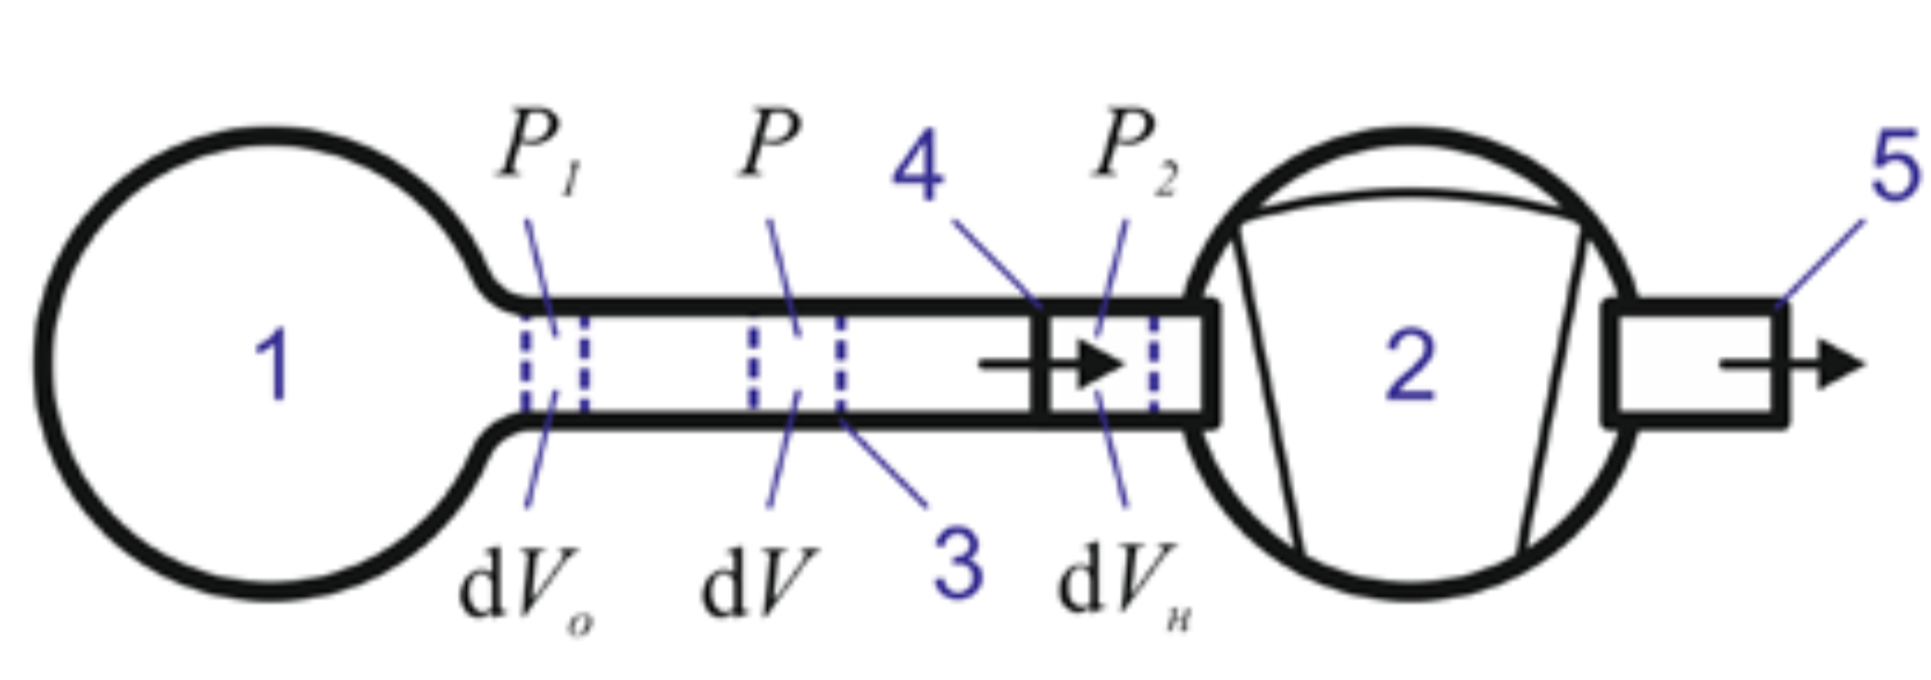
\includegraphics[width=0.8\linewidth]{1} 
    \captionsetup{justification=centering}
    \caption{К определению показателя преломления}
    \label{fig:n}
\end{figure}

Если ограничиться малыми углами, то
\begin{equation}
    \frac{\tg i}{\tg i'} = \frac{d}{d'} \approx \frac{\sin i}{\sin i'}
    = n
    \label{eq:one}
\end{equation}
Измерив расстояние смещения тубуса, можно определить показатель
преломления $n$ пластинки.

\subsubsection*{Определение числовой апертуры объектива микроскопа}
Для определения числовой апертуры необходимо собрать установку,
схема которой показана на \fig{fig:two}

Из представленной на рисунке схемы видно, что $\tg u = m/2L$, откуда
можно найти числовую апертуру $A = \sin u$.


\begin{figure}[H]
    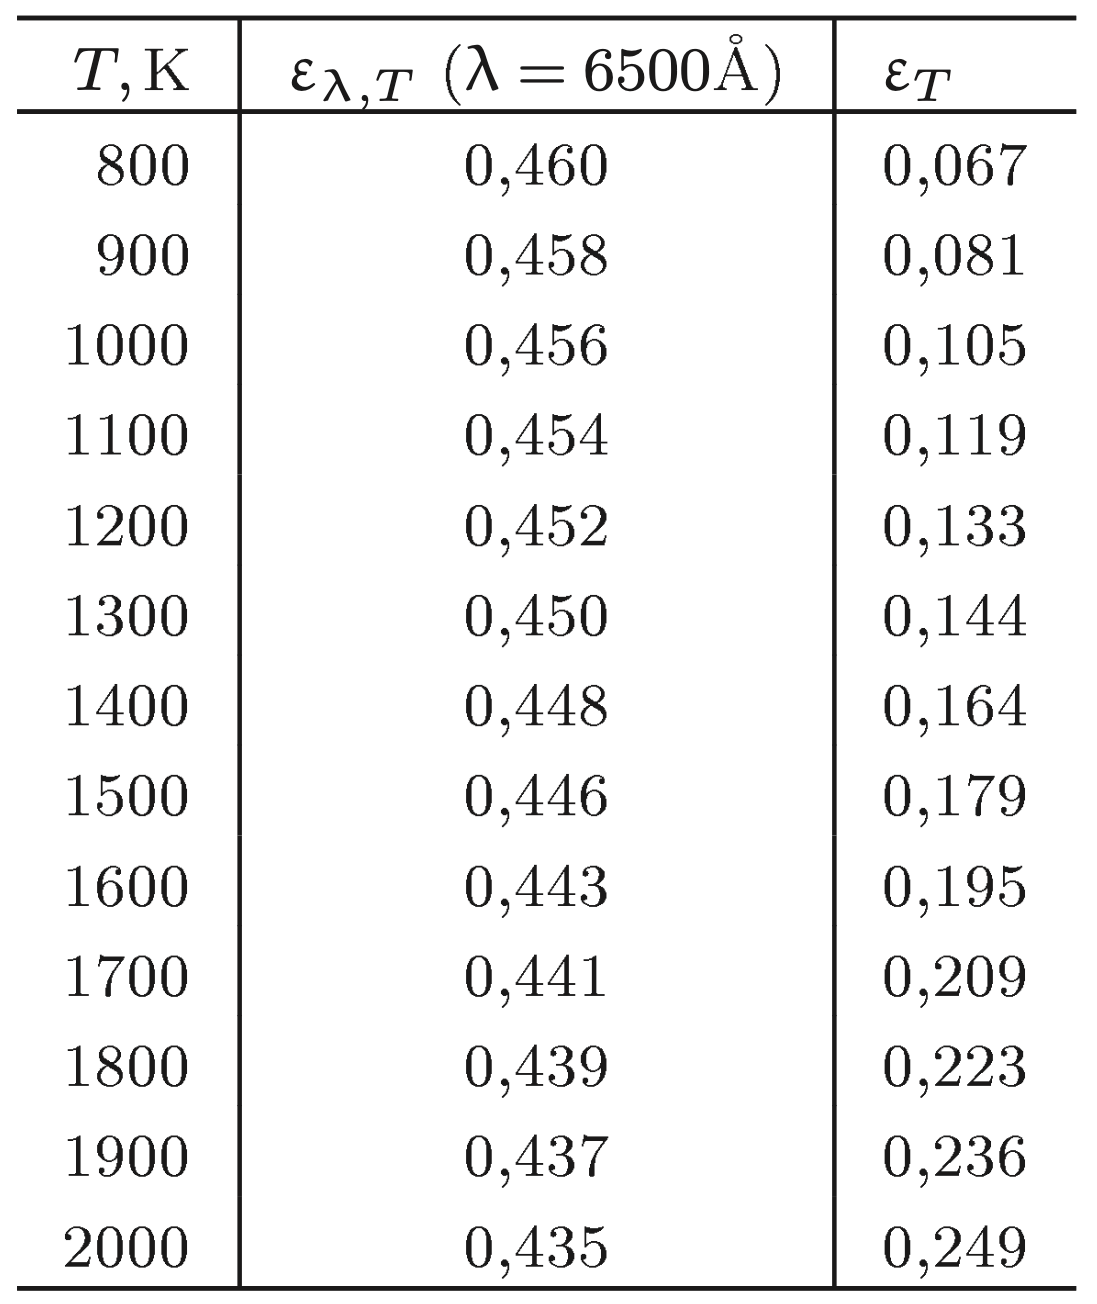
\includegraphics[width=0.9\linewidth]{2} 
    \caption{Схема установки для определения числовой апертуры
    объектива микроскопа. $S$ --- источник света, $P$ --- шкала, $D_1,
D_2, D_3$ --- диафрагмы, $L_1$ --- объектив микроскопа, $t_m$ ---
тубус микроскопа, $L_2$ --- линза с увеличением $\Gamma \approx 1,5$}
\label{fig:two}
\end{figure}

\subsubsection*{Измерение увеличения объектива микроскопа}
Измерение увеличения объектива микроскопа. Если рассматривать объектив
микроскопа как обычную линзу то, из определения поперечного увеличения
и формулы Ньютона следует выражение для поперечного увеличения
\begin{equation}
    \beta = - \frac{f}{x} = - \frac{x'}{f'}
    \label{eq:2}
\end{equation}

Поперечное увеличение объектива может иметь определенное значение
только при заданном значении $x$, а следовательно, и $x'$. Значение
$x'$
определяет, в свою очередь, длину оптического тубуса $\Delta$. Обычно это
значение составляет $160\ \text{мм}$, но в некоторых случаях, например в
измерительных микроскопах, может изменяться в пределах от $130\
\text{мм}$ до $190\ \text{мм}$.

\subsubsection*{Измерение увеличения микроскопа}

\begin{wrapfigure}{r}{0.4\linewidth}
    \vspace{-20pt}
    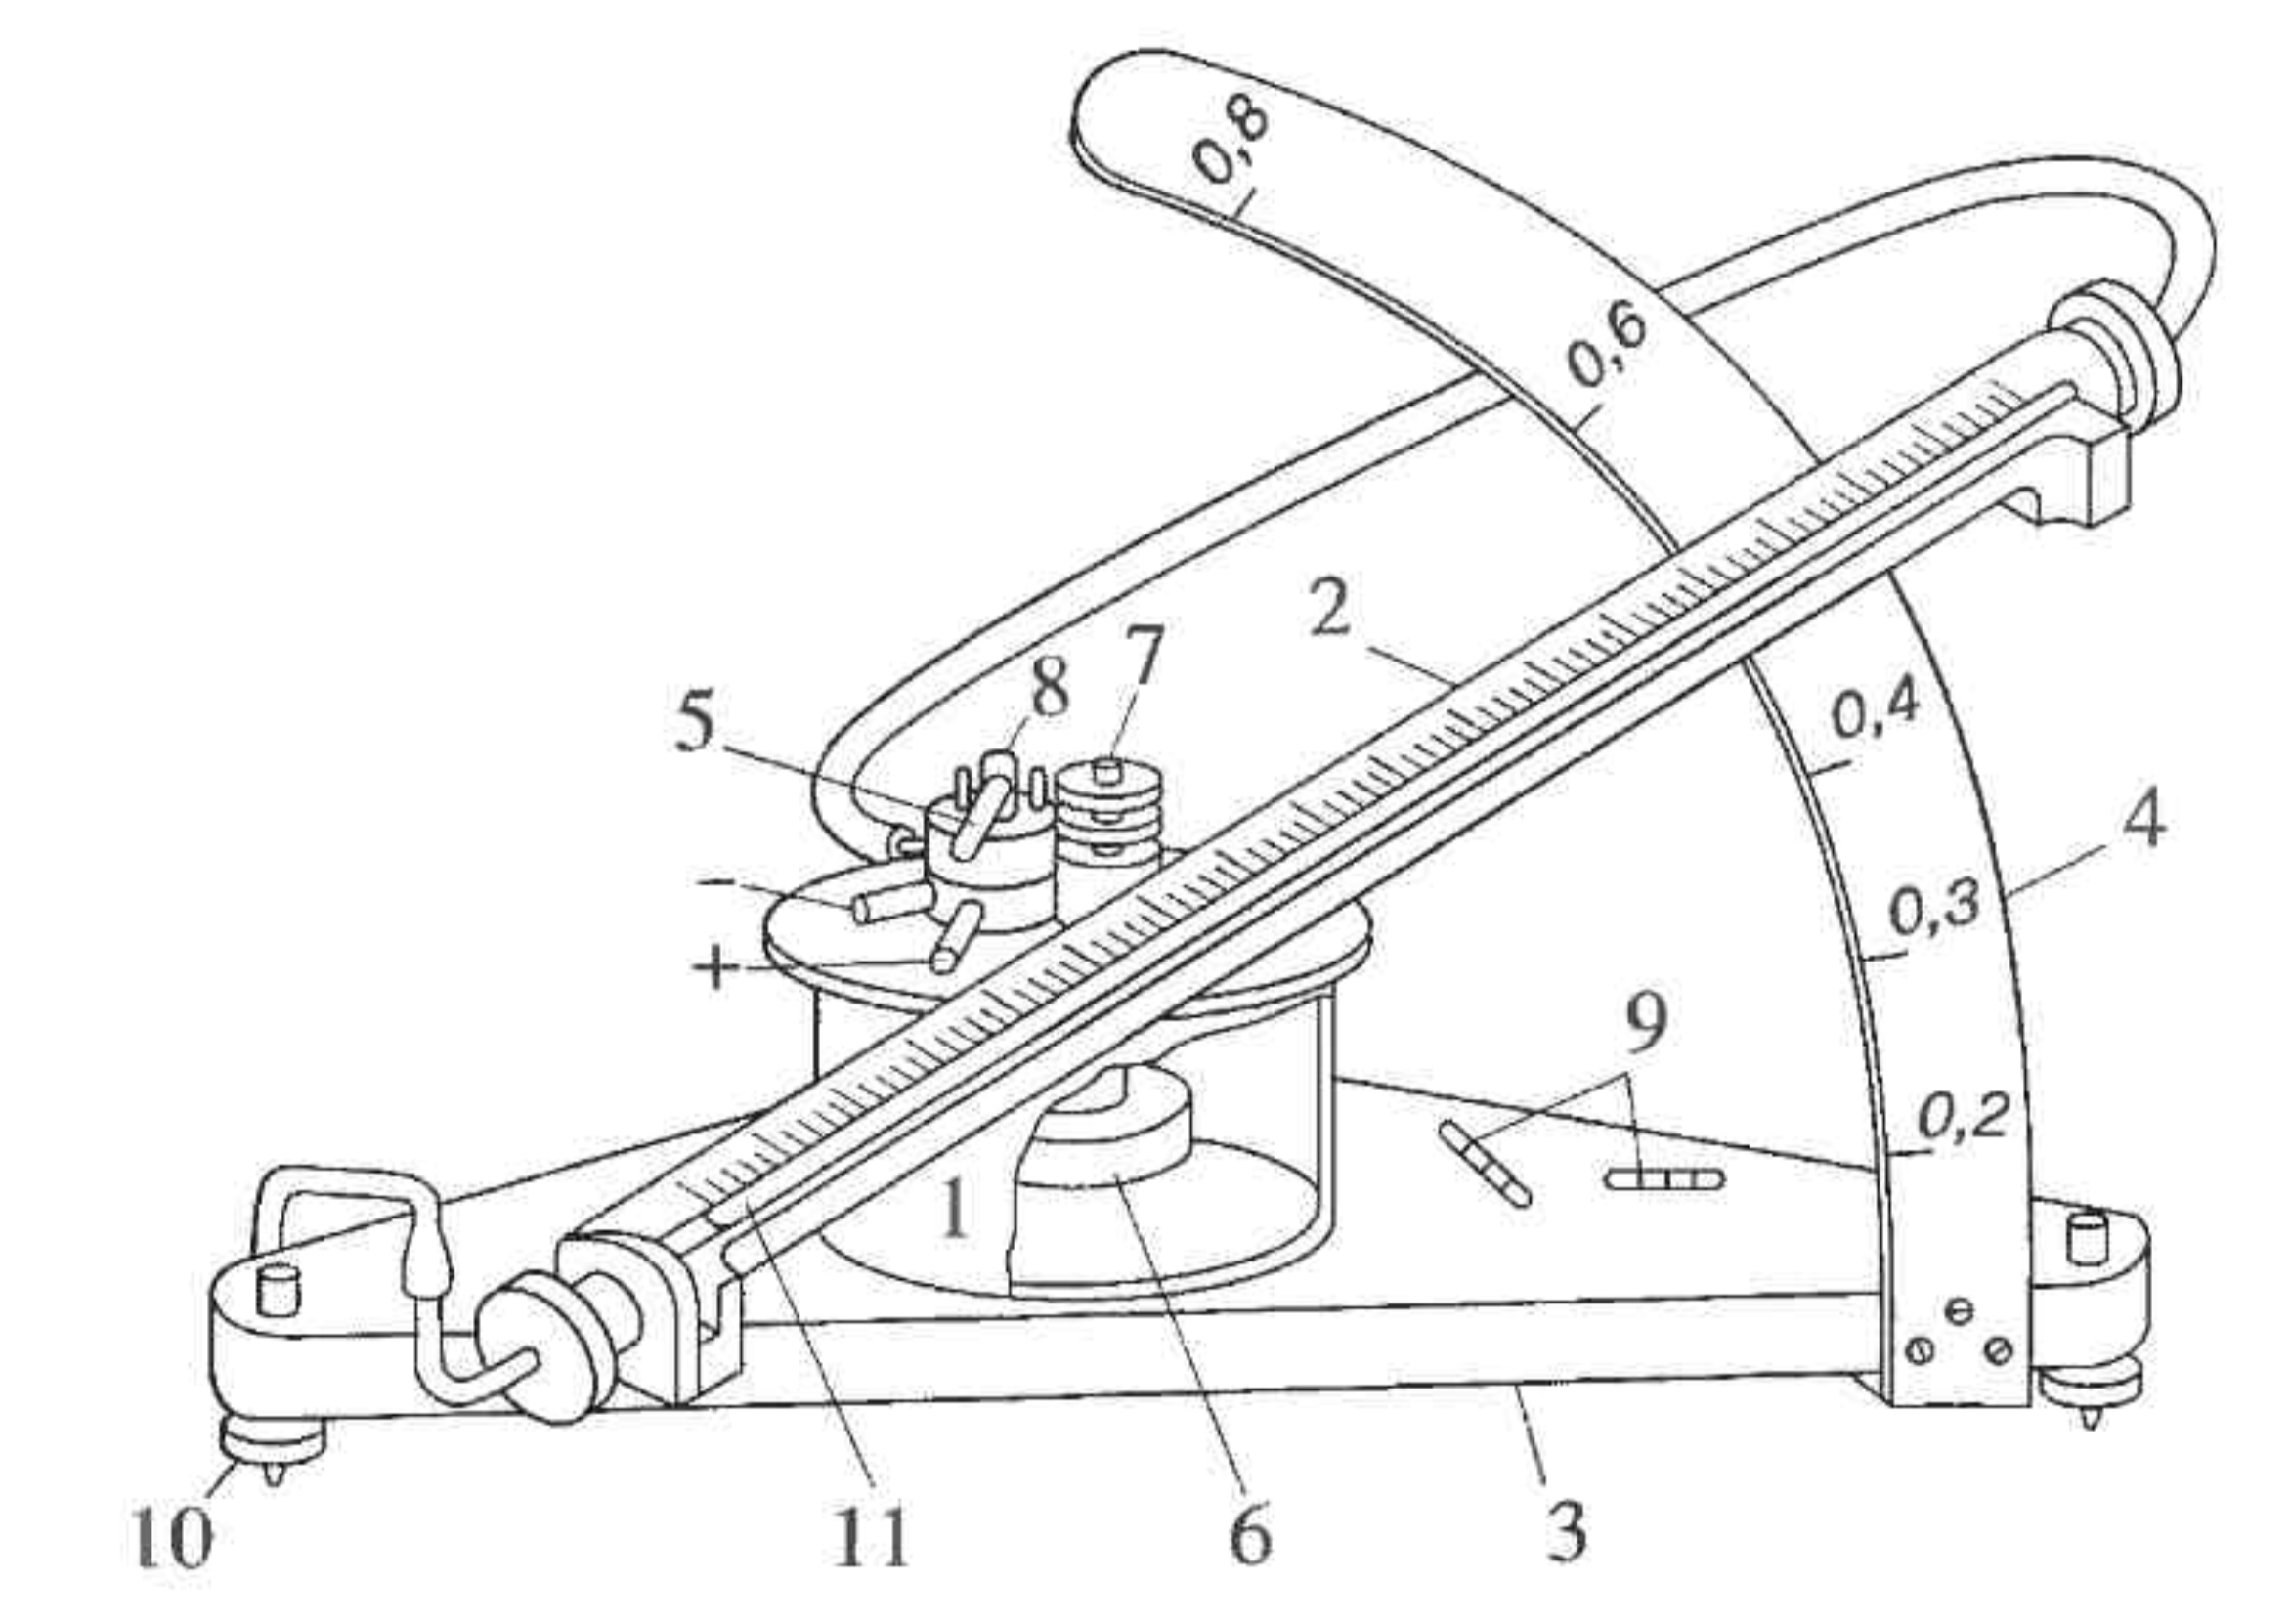
\includegraphics[width=\linewidth]{3}
    \caption{Схема измерения увеличения микроскопа: \textit{1} ---
    тест-объект, \textit{2} --- микроскоп, \textit{3} ---
светоделительный кубик, \textit{4} --- миллиметровая шкала}
\label{fig:three}
\end{wrapfigure}

В некоторых микроскопах специального назначения применяются
нестандартные объективы и окуляры, а также длины тубусов. В этих
случаях для измерения увеличение микроскопа используется следующая
оптическая схема (\fig{fig:three}).

Одна шкала — тест-объект — помещается в предметную плоскость и
рассматривается через микроскоп. Вторая — шкала с миллиметровыми
делениями — рассматривается непосредственно глазом с расстояния
наилучшего зрения. С помощью кубика с полупрозрачным светоделительным
покрытием изображения обеих шкал совмещают и определяют число делений
$n$ объект-микрометра, которое укладываются на $m$ делениях миллиметровой
шкалы.

Тогда для используемого объект-микрометра с ценой деления $0,1\
\text{мм}$ увеличение микроскопа составит 
\begin{equation}
    \Gamma_M = 10 \frac{m}{n}
    \label{eq:Gamma}
\end{equation}

\subsubsection*{Измерение размера выходного зрачка и его удаления от
окуляра микроскопа}
Для измерения размера выходного зрачка и его удаления от окуляра
микроскопа используется универсальный дииаметр Рамсдсиа.

При проведении измерений необходимо осветить объектив микроскопа
расходящимися лучами света. Для этого перед объективом микроскопа
установить матовое стекло, освещенное источником света.

Основание направляющей втулки дииаметра Рамсдсиа приложить к оправе
окуляра микроскопа, а трубку дииаметра передвинуть относительно втулки
до получения резкого изображения апертурной диафрагмы, которое и
является выходным зрачком.

Диаметр выходного зрачка измеряется по стеклянной шкале, а удаление
зрачка отсчитывается но шкале в боковом окне тубуса дииаметра.


\subsubsection*{Измерение разрешающей способности микроскопа}
Для выполнения этого
упражнения установим в микроскоп объектив $3,7^\times$, окуляр
$15^\times$ и
установим длину тубуса микроскопа, равной $160\ \text{мм}$.

Установим перед объективом микроскопа освещенную миру и
наведем микроскоп на нее. Определим номер последнего разрешаемого
элемента.

\subsubsection*{Измерение глубины резко изображаемого пространства}
Для измерения глубины резко изображаемого пространства используется та
же оптическая схема, что и в пункте <<Измерение размера выходного
зрачка и его удаления от окуляра микроскопа>>.

Выберем последний разрешаемый элемент миры и, перемещая миру с помощью
микрометрического винта относительно объектива микроскопа,
зафиксируем положения, при которых изображение штрихов этого
элемента размывается. Разность отчетов по микрометру дает величину
глубины резко изображаемого пространства микроскопа.


\section{Оборудование}
\textbf{В работе используются:} микроскоп <<Биолам>>, измерительный
микроскоп МИР-2, светоделительный кубик, тест-микрометр (макет),
окуляр-микрометр, матовая пластинка с миллиметровой шкалой, лупа с
увеличением $\Gamma = 1,5$, динаметр Рамсдена, источник света. 






\section{Результаты измерений и обработка результатов}
\subsubsection*{Измерение показателя преломления с помощью микроскопа}
Выполним измерения тремя способами 

Поместим на столик микроскопа стеклянную пластинку толщиной $d$ 
(измеренной с помощью микрометра) и, перемещая тубус, навести
микроскоп сначала па верхнюю плоскость пластины (это изображение
пылинок, малых царапин или каких-либо меток), а затем на изображение
нижней поверхности. С помощью микрометрической подачи определим
величину смещения тубуса и рассчитаем значение показателя преломления
пластинки.
\begin{equation*}
    \begin{gathered}
        d = (2,95 \pm 0,05)\ \text{мм}\\
        x = d' = (1,76 \pm 0,04)\ \text{мм}\\
        n = \frac{d}{d'} = 1,68\pm 0,05
    \end{gathered}
\end{equation*}

Навести микроскоп на верхнюю поверхность предметного стекла
(метка $B$ на \fig{fig:n}). Затем на это стекло положить
плоскопараллельную стеклянную пластинку толщиной $d$ и вновь навести
микроскоп на изображение метки $B'$. Изображение $B'$ отстоит от
точки $B$ 
па расстояние $d'' = d-d'$, на которое и необходимо поднять тубус
микроскопа. Поскольку $d'=d/n$, то $d''=d-d/n$. Из последнего
следует
\begin{equation*}
    \begin{gathered}
        y = (0,489 \pm 0,01)\ \text{мм}\\
        n = \frac{d}{d-y}\\
        n = 1,20\pm 0,02
    \end{gathered}
\end{equation*}

Заключительный способ определения $n$ следует из первых двух,
описанных выше. Если использовать выражение $d/d' = n$ и $n =
d/(d-y)$, то получаем
\begin{equation*}
    \begin{gathered}
    n = \left(1+ \frac{y}{x} \right)\\
    n = 1,278 \pm 0,008
    \end{gathered}
\end{equation*}

\subsubsection*{Определение числовой апертуры объектива микроскопа}
Зафиксировав положение объектива, аккуратно удалим из микроскопа
тубус с окуляр-микрометром и снова вставим диафрагму $D_3$. Рассматривая
изображение шкалы $P$, определим число видимых делений $m$. Изображение
шкалы возможно увидеть со сравнительно большого расстояния, однако
выполнить точные измерения в этом случае не представляется возможным.

Измерим расстояние $L$ между шкалой $P$ и диафрагмой $D_2$, рассчитать
числовую апертуру $A$ объектива.

\begin{equation*}
    \begin{gathered}
        m = (40\pm 2)\ \text{мм}\\
        L = (230 \pm 8)\ \text{мм}\\
        \tg u = \frac{m}{2L}\\
        A = \sin u\\
        A = 0,087 \pm 0,005
    \end{gathered}
\end{equation*}

\subsubsection*{Измерение увеличения объектива микроскопа}
C помощью окуляр-микрометра измерим расстояние между изображениями
штрихов тест-объекта и рассчитаем увеличение объектива микроскопа. В
4 деления окуляра-микрометра укладывается 9 делений тест-объекта.
\begin{equation*}
    \begin{gathered}
        \beta = 4,4 \pm 0,1 
    \end{gathered}
\end{equation*}

\subsubsection*{Измерение увеличения микроскопа}
Измерим увеличение микроскопа с двумя различными окулярами и при
различной длине тубуса (130 мм, 160 мм, 190 мм).

\renewcommand{\arraystretch}{1.3}

\begin{table}[H]
\centering
\begin{tabular}{|c|c|c|}
    \hline 
    Окуляр & \specialcell{Длина тубуса,\\[-9pt] $\text{мм}$} & $\Gamma_M$ \\ \hline 
    \multirow{3}{*}{$\times 15$} & 130 & 34 \\ \cline{2-3} 
    & 160 & 44\\ \cline{2-3} 
    & 190 & 60\\ \hline 
    \multirow{3}{*}{$\times 10$} & 130 & 30 \\ \cline{2-3} 
    & 160 & 42 \\ \cline{2-3}
    & 190 & 50 \\ \hline  
\end{tabular}
\caption{Измерение увеличения микроскопа}
\end{table}

\subsubsection*{Измерение размера выходного зрачка и его удаления от
окуляра микроскопа}

Диаметр выходного зрачка: 
\[
    d = (1,9 \pm 0,2)\ \text{мм}
\]

Удаления зрачка 

\[
    \Delta l = 2,7\ \text{см}
\]

Диаметр входного зрачка

\[
    d' = (0,051\pm 0,008)\ \text{мм}
\]

\subsubsection*{Измерение разрешающей способности микроскопа}
Номер последнего разрешаемого элемента миры равен 20.  По таблице
определим значение разрешающей способности микроскопа

\[
    L = 33\cdot 10^{-4}\ \text{мм}
\]

\subsubsection*{Измерение глубины резко изображаемого пространства}
Глубина резко изображаемого пространства равна

\[
    x = (0,43\pm 0,03)\ \text{мм}
\]

Теоретическая оценка значения

\[
    x_{\text{т}} = 0,01\ \text{мм}
\]


\section{Обсуждение результатов и выводы}
В работе были изучены принципы построения микроскопических систем и
методы измерения их основных характеристик.

Была определена числовая апертура объектива микроскопа 

\[
    A = 0,087 \pm 0,005
\]

Проведено измерение увеличения объектива микроскопа 

\[
    \beta = 4,4 \pm 0,1
\]

Значение, указанное на объективе:

\[
    \beta_\text{т} = 3,7
\]

Измерено увеличение микроскопа с двумя различными окулярами и при
различной длине тубуса \textsl{табл. 1}

Был измерен диаметр выходного зрачка 
\[
    d = (1,9\pm 0,2)\ \text{мм}
\]

И вычислен размер входного 
\[
    d' = (0,051 \pm 0,009) \text{мм}
\]

Разрешающая способность микроскопа равна

\[
    L = 33 \cdot 10^{-4}\ \text{мм}
\]

Измерена глубина резко изображаемого пространства

\[
    x = (0,43\pm 0,03)\ \text{мм}
\]

Что значительно превосходит теоретическую оценку

\[
    x_\text{т} = 0,01\ \text{мм}
\]




\end{document}
